%!TEX root = ../../main.tex

\newcommand{\importGQL}[2]{
    \lstinputlisting[
        caption={#2},
        label={ls:gql:#1}
    ]{src/code/#1.gql}   
}

\newcommand{\importHS}[2]{
    \lstinputlisting[
        language={haskell},
        caption={#2},
        label={ls:hs:#1}
    ]{src/code/#1.hs}   
}

\newcommand{\expr}[1]{\hspace{0.2mm}\mbox{\textcolor{green!35!blue!55!black}{\texttt{#1}}}}

\newcommand{\refGQL}[1]{Listing \ref{ls:gql:#1}}
\newcommand{\refHS}[1]{Listing \ref{ls:hs:#1}}

\section{Background}

\begin{frame}\frametitle{Haskell}

    \footnotesize
    \begin{block}{Haskell}
        Haskell is a non-strict, purely functional language with static typing and algebraic data types. It is a rich language that offers useful features such as currying, infix-prefix operations, anonymous functions, list comprehensions, and monads. In order to easily distinguish constructors, it allows only capitalized constructors and disallows them for variables. Besides, the language contains type system extensions like polymorphic recursion, higher-rank types, lexically scoped type variables, generic programming, template meta-programming,  and much more. Many developers think that Haskell programs look nice~\cite{history-of-haskell}.
    \end{block}

    \begin{block}{The following topics outline Haskell's main goals and principles}
    
        \begin{itemize}
            \item Haskell is lazy: 
            Laziness was indeed the primary concern in Haskell's design. Technically, Haskell is a non-strict semantic language; lazy evaluation is merely an implementation technique for a non-strict language.  However, since laziness has its price 
            , the language also offers some strict features~\cite{history-of-haskell}.
    
            \item Haskell is pure: Due to laziness, the evaluation sequence is demand-oriented, a function call can no longer guarantee reliable performance of side effects. Consequently, the pure design is inevitable. Since input and output operations can be painfully complicated without side effects, the Haskell developers have developed a new approach called monadic IO, which is one of Haskell's most important contributions to the world~\cite{history-of-haskell}.
        \end{itemize}

    \end{block}

\end{frame}

\begin{frame}\frametitle{Algebraic Data Types}

An algebraic data type is the sum of one or more alternatives, where each alternative is a product of zero or more fields (Haskell also allows a sum of zero alternatives, the so-called empty type)~\cite{history-of-haskell}. 

Algebraic data types and pattern matching are fundamental to most modern functional languages~\cite{trees-that-grow}. Using pattern matching against algebraic data types improves readability significantly~\cite{history-of-haskell}.
    

Listing  declares \expr{Maybe} as data type, with two data constructors, \expr{Nothing} and \expr{Just}. The values of type \expr{Maybe} take one of two forms: either \expr{Nothing} or \expr{Just x}. Constructors can be used in pattern matching to decompose both a value of type and an expression~\cite{history-of-haskell}. 
    
\importHS{maybe}{Algebraic Data Types~\cite{history-of-haskell}}

algebraic data types also have their limitations. Once a data type is defined and compiled, its definition cannot be extended by adding new data constructors (or new fields)~\cite{trees-that-grow}.

\end{frame}

\begin{frame}\frametitle{Records}
    
    Early versions of Haskell provided only positional notation and pattern matching to build and decompose user-defined data types. This positional notation is cumbersome and error-prone for handling data types with many components, which is quite common in real-world applications. Therefore, later versions of Haskell introduced minimalistic record syntax as a labeled field~\cite{lw-ext-records, history-of-haskell}.
The record system provides syntactic sugar for what might 
otherwise be written using ordinary, positional, 
algebraic data type declarations~\cite{lw-ext-records}. For example, 
the data type \expr{Deity} declares a regular algebraic data type, 
but at the same time, 
constructor field accessors and modifiers. 

\importHS{records}{Haskell Record}

Record characteristics bring significant advantages and greatly simplify programming with data structures that have many components. Since the individual components are accessed by name (not by position), the fields' ordering is not crucial~\cite{lw-ext-records}.
In \refHS{record-values}, for example, 
the same record value can be written either way.

However, records also introduce some considerable problems; for example, 
no field name can be used in more than one data type~\cite{lw-ext-records}.
Another weakness of Haskell record systems is that there is no support for extensibility. 
There are no operators for adding and removing fields in a record~\cite{poly-ext-records, hlist}. 
Moreover, labels are not first-class citizens, 
meaning we cannot reuse labels between different record types, 
nor can we treat labels as data~\cite{hlist}.
This missing feature gave rise to many discussions and proposals to support polymorphic extensible records with different approaches~\cite{history-of-haskell, poly-ext-records, hlist, basic-tlp}.

\end{frame}

\begin{frame}\frametitle{Monads}

Besides the type classes, the monads are among the most characteristic features in Haskell. Haskell represents monads with the help of type classes. The class monad allows every type constructor, which has accordingly typed unit and binding operators, to be a monad. 
This states that we can write useful monadic combinators, which work for every monad. 
This combination of monads and type classes made each other much more attractive and gave rise to entire Haskell libraries with monadic functions that work for any monad~\cite{history-of-haskell}. 

\importHS{monad}{Monad in Haskell~\cite{history-of-haskell}}

Pure languages facilitate changes by making the data visible on which each operation depends. However, a seemingly small change may require more extensive restructuring than impure functions.  Programming with monads solves this inflexibility and brings properties that are characteristic only of impure functions~\cite{essence-of-fp}.

The concept of monads comes from category theory but has come to represent a kind of programming pattern~\cite{essence-of-fp,history-of-haskell}. It  is formed by a type constructor \expr{M} and a pair of functions, \expr{unitM} (also \expr{return}) and \expr{bindM} (also \expr{>>=})~\cite{history-of-haskell,essence-of-fp}. Listing \ref{ls:hs:monad} represents these types:

The type \expr{M a} is a computation that returns a value of type \expr{a} and possibly performs some side effects~\cite{history-of-haskell}. The purpose of \expr{unitM} and \expr{bindM} is to push a value into computation and to evaluate a computation, yielding a value~\cite{essence-of-fp}.

Say that \expr{comp1} is an expression of type \expr{M a} and \expr{comp2} is an expression of type \expr{M b}. Then with a free variable \expr{x} of type \expr{a} the expression \expr{bindM comp1 (x -> comp2)} has type \expr{M b}, where expression performs the computation indicated by \expr{comp1}, binds the value returned to \expr{x}, and performs the computation indicated by \expr{comp2}~\cite{history-of-haskell}.

In some languages, types do not indicate the presence of the side effects: there, \expr{comp1} is of type \expr{a} instead of \expr{M a} and \expr{comp2} is of type \expr{b} instead of \expr{M b}. Therefore it is impossible to determine from the signature if the function has side effects. Consequently, language uses a single built-in notion of computation and sequencing. In contrast, the monads leave quite a lot of freedom to define the operations and their order of execution~\cite{history-of-haskell}.

There are several different instances of monads handling side effects. For example, a state transformer enables the sharing of a state in a program. It accepts a state that can be read or modified by the computations. A simplified version of a state transformer is a state reader. It accepts a state, but the computations never change it. One of the well-known variants of the monad is a list that stores values of a specific type ~\cite{history-of-haskell}.


\end{frame}

\begin{frame}\frametitle{Datatype-Generic Programming}
    
 For some domains, such as encoding and decoding, most of the procedures are the same. However, the data types differ, requiring the complete functionalities to be rewritten. Datatype-generic programming is a technique for tackling this issue by automatically generating programs depending on these data types~\cite{comparing-generic-approaches, datatype-generic-programming}. 
    It enables writing single (called generic or polytypic) functions that address various cases and types. The standard examples are parsing,  serialization, or comparing of data types~\cite{derivable-type-classes}.
    
    The term "generic" is an overused adjective in computer science. 
    Various programming languages provide generic packages 
    representing different ideas. 
    Usually, it indicates that a concept allows abstractions over a larger class of entities. 
    However, most often, "generic" refers to parametric polymorphism, 
    ad hoc polymorphism, inheritance, or meta-programming~\cite{optimizing-generics,datatype-generic-programming}.  
    For this work, the term "generic programming" means a form of programming in which a function takes a type as an argument and performs appropriate behavior depending on its structure. 
    This kind of generic programming is also called datatype-generic programming~\cite{comparing-generic-approaches, datatype-generic-programming}.
    It increases the reliability of programs by reducing code duplication and improving reusability and modularity~\cite{optimizing-generics}.
    The core concept is that it makes programming languages flexible while still guaranteeing safety~\cite{datatype-generic-programming}.
    There are many datatype-generic programming approaches that vary in sophistication and target audience~\cite{comparing-generic-approaches, optimizing-generics}.
    In this section, we will discuss the standard Haskell approach.
    
    Let us examine the data type  \expr{Computation} in \refHS{deriving-node}. 
    To define the equality instance for this data type, we must first check whether both values have the same constructor. In the second step, we must check whether each field of the constructors is equal, which requires an equality instance for its type variable \expr{a}. Since the equality check is programmable, Haskell provides a so-called "deriving" clause that instructs the compiler to generate the "boilerplate" for equality~\cite{derivable-type-classes, meta-hs}. 
    
    \importHS{generics}{Generic Deriving}
    
    However, if we want to define our derivable programs like encoders or decoders for arbitrary types, we can use the Haskell package GHC.Generics~\cite{ghc-generics}. The basic idea behind it is to represent all types and values by a small set of data types, which are also called generic representation types. They are the building blocks of the structural representation of all other types~\cite{optimizing-generics}.
    Using the \expr{from} and \expr{to} functions, the user can convert arbitrary types to their generic representation, operate on them, and convert them back to their original types~\cite{optimizing-generics,history-of-haskell, ghc-generics}.

\end{frame}

\begin{frame}{GraphQL}

    \footnotesize

    \begin{block}{Was ist GraphQL?}
        GraphQL ist eine API-Abfragesprache zur Lösung der Effizienzprobleme der Kommunikation\cite{gql-iot}.         
    \end{block}

    \begin{block}{von Facebook Entwicklt}
        Es wurde drei Jahre lang intern bei Facebook entwickelt und seine Spezifikation und seine Referenzimplementierung 2016 veröffentlicht.
        \cite{initial-analysis-of-gql}
    \end{block}

    \begin{block}{GraphQL als aktueller Trend}
        Seit ihrem ersten Erscheinen hat sie ein reiches Open-Source-Ökosystem und das Vertrauen von Unternehmen aus verschiedenen Sektoren gewonnen. z.B: (GitHub), Unterhaltung (Netflix), Finanzen (PayPal), Reisen (KLM), etc \cite{morph-gql-1,gql-healthcare}.
    \end{block}

\end{frame}






% \section{Morpheus GraphQL}
% \setBGColor{white}
% \begin{frame}{Morpheus GraphQL}
%     \begin{figure}
%         \centering
%         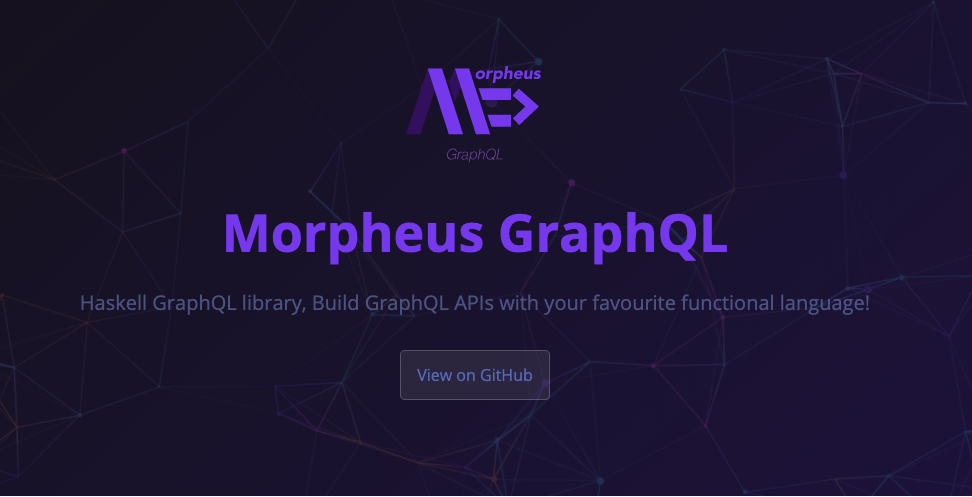
\includegraphics[width=1.1\textwidth]{assets/img/morpheus-graphql-bg.png}
%     \end{figure}
% \end{frame}